\documentclass[a4paper,11pt]{article}

\usepackage[margin=2.5cm]{geometry}
\usepackage[T1]{fontenc}
\usepackage[utf8]{inputenc}
\usepackage[english]{babel}
\usepackage{lmodern}
\usepackage{microtype}
\usepackage{graphicx}
\graphicspath{{../figures/}{part1/figures/}}
\usepackage{booktabs}
\usepackage{tabularx}
\usepackage{array}
\usepackage{float}
\usepackage{hyperref}
\usepackage{xcolor}
\usepackage{caption}
\usepackage{listings}

\hypersetup{
  colorlinks=true,
  linkcolor=blue!50!black,
  urlcolor=blue!50!black,
  pdftitle={IoT Challenge 2 -- Part 1},
  pdfauthor={Tommaso Neri}
}

\lstset{
  basicstyle=\ttfamily\small,
  columns=fullflexible,
  keepspaces=true,
  frame=single,
  breaklines=true,
  showstringspaces=false
}

\captionsetup{font=small,labelfont=bf}
\setlength{\parindent}{0pt}
\setlength{\parskip}{0.55em}
\renewcommand{\arraystretch}{1.18}
\linespread{1.04}
\setcounter{tocdepth}{2}

\newcommand{\coursename}{Internet of Things Lab}
\newcommand{\challengename}{IoT Challenge \#2 -- Network Trace Analysis}
\newcommand{\authorname}{Tommaso Neri}
\newcommand{\personcode}{10817232}
\newcommand{\teammates}{N/A (Single)}
\newcommand{\answer}[1]{\textbf{\textcolor{red}{#1}}}
\newcommand{\code}[1]{\texttt{#1}}
\newcommand{\scriptpath}[1]{\path{#1}}

\title{\challengename}
\author{
  \authorname\\
  Person Code: \personcode\\
}
\date{\today}

\begin{document}

\maketitle
\thispagestyle{empty}

\begin{center}
\begin{tabular}{ll}
\toprule
Course & \coursename \\
Challenge & Part 1 -- CQ1 to CQ8 \\
Input traces & \code{A.pcapng}, \code{B.pcapng} \\
Main tools & Wireshark/TShark, Python scripts \\
\bottomrule
\end{tabular}
\end{center}

\vspace{1em}

\newpage
\tableofcontents
\newpage

\section{Method Notes}
Malformed packets are ignored in every answer. The final values are highlighted in
red, and the scripts used for verification are reported in each section.

When the question depends on a protocol exchange, I do not count packets only from a
broad display filter. I first select candidate packets, then verify the actual
relationship using protocol fields such as token, MID, direction, endpoint and
message type.

\section{Final Answers}
\begin{table}[H]
\centering
\caption{Summary of the final answers.}
\begin{tabularx}{\textwidth}{@{}l l X@{}}
\toprule
\textbf{Question} & \textbf{Answer} & \textbf{Meaning} \\
\midrule
CQ1a & \answer{MID 30800} & NON DELETE request to \code{coap.me} with a proper successful DELETE response. \\
CQ1b & \answer{0} & CQ1a requests whose later GET to the same resource returns \code{4.04 Not Found}. \\
CQ2 & \answer{1} & Resource with equal non-zero counts of unsuccessful CON POST and PUT requests. \\
CQ3a & \answer{10} & Separate Observe notifications for \code{/dining\_room/temperature}. \\
CQ3b & \answer{5} & CQ3a notifications that generated ICMP Port Unreachable. \\
CQ4 & \answer{0} & MQTT-SN messages sent from the local broker to clients. \\
CQ5 & \answer{1} & Subscriber receiving a Last Will through a wildcard subscription. \\
CQ6a & \answer{5} & HiveMQ clients that erased a retained value with an empty retained PUBLISH. \\
CQ6b & \answer{2} & CQ6a clients with client identifier longer than 7 bytes. \\
CQ7 & \answer{9} & Local MQTT SUBSCRIBE requests with at least two wildcards. \\
CQ8a & \answer{439} & Local broker PUBLISH messages in \code{A.pcapng}. \\
CQ8b & \answer{534} & Local broker PUBLISH messages in \code{B.pcapng}. \\
\bottomrule
\end{tabularx}
\end{table}

\newpage
\section{CoAP Questions}

\subsection{CQ1 -- CoAP DELETE to \code{coap.me}}
\subsubsection{Question}
CQ1a asks for the MIDs of non-confirmable DELETE requests to
\code{coap.me} that receive a successful response. CQ1b asks how many of those
requests obtained the desired DELETE outcome.

\subsubsection{Script and Filter}
\scriptpath{part1/scripts/cq1_a_delete_success.py}

\begin{lstlisting}
coap && !_ws.malformed && coap.type == 1 && coap.code == 4 &&
ip.dst == 134.102.218.18 && udp.dstport == 5683
\end{lstlisting}

For the CQ1b validation GET on the same resource:
\begin{lstlisting}
coap && !_ws.malformed && coap.code == 1 &&
ip.dst == 134.102.218.18 && udp.dstport == 5683 &&
coap.opt.uri_path_recon == "/validate"
\end{lstlisting}

\subsubsection{Reasoning}
The destination is the public CoAP endpoint \code{134.102.218.18:5683}. I match each
candidate DELETE request with the first later CoAP response having a non-empty
matching token, reversed client/server endpoints, and a non-empty response code.
Empty tokens are ignored because they are valid in CoAP but unsafe as a correlation
key in a capture-wide search.

For this request, ``successful'' is interpreted as a method-correct DELETE success:
\code{2.02 Deleted}, exported by TShark as \code{coap.code == 66}. This avoids
counting a generic response that does not express a successful DELETE. The request
MID is reported for CQ1a, but it is not used as the only matching key because the
CoAP token and endpoints identify the request/response relation more reliably for
this NON exchange.

For CQ1b, the desired final outcome is checked with the later GET to the same
resource. The deleted resource should no longer be available, so the follow-up GET
must return \code{4.04 Not Found}.

\subsubsection{Result}
\begin{table}[H]
\centering
\caption{CQ1 matched DELETE exchange.}
\begin{tabularx}{\textwidth}{@{}r r X r l@{}}
\toprule
Request frame & Request MID & Token & Response frame & Response code \\
\midrule
11075 & \answer{30800} & \code{880f30d8b543d6f7} & 11078 & \code{2.02 Deleted} \\
\bottomrule
\end{tabularx}
\end{table}

\begin{table}[H]
\centering
\caption{CQ1b follow-up availability check.}
\begin{tabular}{lrrl}
\toprule
Resource & GET frame & Response frame & Response code \\
\midrule
\code{/validate} & 11363 & 11364 & \code{2.05 Content} \\
\bottomrule
\end{tabular}
\end{table}

Among 20 candidate NON DELETE requests, only this exchange matches a proper DELETE
success response. The later GET to the same resource is frame 11363 and its response
at frame 11364 is \code{2.05 Content}, not \code{4.04 Not Found}. Therefore CQ1a is
\answer{MID 30800} and CQ1b is \answer{0}.

\subsection{CQ2 -- Unsuccessful CON POST/PUT Requests}
\subsubsection{Question}
Count the local CoAP resources that received the same non-zero number of unique
unsuccessful confirmable POST and PUT requests.

\subsubsection{Script and Filter}
\scriptpath{part1/scripts/cq2_a_coap_post_put.py}

\begin{lstlisting}
coap && !_ws.malformed && coap.type == 0 &&
(coap.code == 2 || coap.code == 3) &&
ip.dst == 127.0.0.1 && udp.dstport == 5683
\end{lstlisting}

\subsubsection{Reasoning}
The local CoAP server is \code{127.0.0.1:5683}; public \code{coap.me} traffic is
therefore explicitly excluded (including it would erroneously add 36 requests), as 
the question strictly asks for requests to the local server. A request is counted 
only after its response has been matched: piggybacked responses require token, 
reversed endpoints and the same MID, while separate responses use the same non-empty 
token and reversed endpoints. Empty ACKs with \code{coap.code == 0} are skipped 
because they acknowledge the CON message but do not state success or failure.

Unsuccessful responses are the CoAP client/server error classes, \code{4.xx} and
\code{5.xx}. Different requests are counted separately even when they receive the
same error code; retransmissions are deduplicated by method, resource, MID, token
and endpoints.

\subsubsection{Result}
\begin{table}[H]
\centering
\caption{CQ2 resource satisfying the POST/PUT condition.}
\begin{tabular}{lcc}
\toprule
Resource & Unsuccessful POST & Unsuccessful PUT \\
\midrule
\code{/dining\_room} & 1 & 1 \\
\bottomrule
\end{tabular}
\end{table}

Only \code{/dining\_room} has equal non-zero counts, so the answer is \answer{1}.

\subsection{CQ3 -- CoAP Observe Notifications}
\subsubsection{CQ3a Question}
Count the separate Observe notifications containing values for
\code{/dining\_room/temperature}, ignoring retransmissions.

\subsubsection{Script and Filters}
\scriptpath{part1/scripts/cq3_a_observe_temperature.py}

\begin{lstlisting}
coap && !_ws.malformed && coap.code == 1 && coap.opt.observe == 0 &&
coap.opt.uri_path_recon == "/dining_room/temperature"
\end{lstlisting}

\begin{lstlisting}
coap && !_ws.malformed && coap.opt.observe && json.value.string &&
udp.srcport == 5683
\end{lstlisting}

\subsubsection{Reasoning}
The Observe registration is frame 4343, from
\code{127.0.0.1:48049} to \code{127.0.0.1:5683}, with token \code{89b9}. Only later
server-to-client packets with the same token, the same resource path, a
\code{2.05 Content} response code and a temperature payload are considered.

Frame 4344 confirms the registration and already carries a valid resource value, but
it is not counted here because CQ3a asks for \emph{separate} notifications (counting
it would incorrectly yield 11 instead of 10). I count only later Observe messages 
with a different MID from the registration request.
Retransmissions and duplicate loopback views are removed using Wireshark fields and
the duplicated loopback IP pattern.

\subsubsection{Result}
\begin{table}[H]
\centering
\caption{CQ3 Observe exchange summary.}
\begin{tabularx}{\textwidth}{@{}l p{4.2cm} X@{}}
\toprule
Item & Frame(s) & Meaning \\
\midrule
Registration & 4343 & GET Observe for \code{/dining\_room/\allowbreak temperature}, token \code{89b9}. \\
Initial response & 4344 & Valid value, but not a separate notification. \\
Acknowledged counted notifications & 4620, 5098, 5623, 8509, 9414 & Later Observe CON messages with same token, different MID, and an empty ACK from the observer. \\
Unreachable counted notifications & 9866, 10573, 11220, 11917, 12782 & Later Observe CON messages with same token and different MID. Each one generates ICMP Port Unreachable. \\
\bottomrule
\end{tabularx}
\end{table}

The CQ3a answer is \answer{10}.

\subsubsection{CQ3b Question}
Count how many notifications from CQ3a are useless.

\subsubsection{Reasoning and Result}
For the purpose of the challenge, I treat a CQ3a notification as useless only when
it is sent over the network but not successfully received or processed. Since the
counted notifications are Confirmable CoAP messages, an empty ACK from the observer
is evidence of successful processing, while ICMP Port Unreachable is evidence that
the notification was sent to a no longer reachable client. Retransmissions are
still excluded, because CQ3b refers only to the notifications counted in CQ3a.

The first five counted notifications have ACKs at frames 4624, 5099, 5629, 8510
and 9415. The last five counted notifications generate ICMP Port Unreachable at
frames 9867, 10574, 11221, 11918 and 12783. No repeated-value notifications are
present. The CQ3b answer is \answer{5}.

\newpage
\section{MQTT-SN Question}

\subsection{CQ4 -- Broker-to-Client Messages}
\subsubsection{Question}
Count MQTT-SN messages received by clients from the local broker listening on UDP
port 1885.

\subsubsection{Script and Filter}
\scriptpath{part1/scripts/cq4_a_mqttsn_local.py}

\begin{lstlisting}
mqttsn && !icmp && !_ws.malformed
Decode-as: udp.port==1885,mqttsn
\end{lstlisting}

\subsubsection{Reasoning}
UDP port 1885 must be decoded as MQTT-SN before counting. ICMP is excluded because
Wireshark may dissect the original embedded UDP payload inside ICMP errors; those
embedded payloads are not messages received by clients.

The question asks for messages from the broker to clients, so the broker must be the
sender: \code{udp.srcport == 1885}. After the decode-as step, the capture contains
219 MQTT-SN messages in total, but they are all directed from clients to the broker
with \code{udp.dstport == 1885}. The broker never responds (all packets receive an ICMP Destination Unreachable 
response, confirming the broker is offline), so none have source port 1885. A common 
error is counting all messages on port 1885 (which would give 219), but this 
ignores the strict \emph{received by the clients} direction requirement.

\subsubsection{Result}
\begin{table}[H]
\centering
\caption{CQ4 MQTT-SN direction check.}
\begin{tabular}{lc}
\toprule
Direction & Messages \\
\midrule
Client to broker, \code{udp.dstport == 1885} & 219 \\
Broker to client, \code{udp.srcport == 1885} & \answer{0} \\
\bottomrule
\end{tabular}
\end{table}

The answer is \answer{0}.

\newpage
\section{MQTT Questions}

\subsection{CQ5 -- Last Will Delivered Through Wildcards}
\subsubsection{Question}
Count MQTT subscribers that receive a Last Will message because of a subscription
containing at least one wildcard.

\subsubsection{Script and Filters}
\scriptpath{part1/scripts/cq5_b_last_will_wildcards.py}

\begin{lstlisting}
mqtt && !_ws.malformed && mqtt.msgtype == 1 &&
mqtt.conflag.willflag == 1
\end{lstlisting}

\begin{lstlisting}
mqtt && !_ws.malformed && mqtt.msgtype == 8 &&
(mqtt.topic contains "+" || mqtt.topic contains "#")
\end{lstlisting}

\begin{lstlisting}
mqtt && !_ws.malformed && mqtt.msgtype == 3 && tcp.srcport == 1883
\end{lstlisting}

\subsubsection{Reasoning}
The script joins three facts from the capture: the Last Will declared in CONNECT, the
subscriber's previous wildcard SUBSCRIBE, and the broker-to-client PUBLISH that
delivers the Will topic and payload. A subscriber is counted only if its wildcard
filter matches the Will topic and the delivery happens after the subscription.

\subsubsection{Result}
\begin{table}[H]
\centering
\caption{CQ5 wildcard Last Will delivery.}
\begin{tabularx}{\textwidth}{@{}l X@{}}
\toprule
Field & Value \\
\midrule
Subscriber & \code{zmjnxudohrkaegmh} \\
Wildcard subscription & \code{university/\#} \\
Delivered Last Will topic & \code{university/\allowbreak department12/\allowbreak room1/\allowbreak temperature} \\
Delivery frame & 6564 \\
\bottomrule
\end{tabularx}
\end{table}

Four Last Wills are declared, but only one is delivered through a matching wildcard
subscription. The answer is \answer{1}.

\subsection{CQ6 -- Retained Value Erasure on HiveMQ}
\subsubsection{CQ6a Question}
Count different MQTT clients that sent at least one message to erase a previously
retained value in a topic in the public HiveMQ broker.

\subsubsection{Script and Filters}
\scriptpath{part1/scripts/cq6_b_retained_erase.py}

\begin{lstlisting}
dns && dns.qry.name == "broker.hivemq.com"
\end{lstlisting}

\begin{lstlisting}
mqtt && !_ws.malformed && mqtt.msgtype == 3 && mqtt.retain == 1
\end{lstlisting}

\subsubsection{Reasoning}
HiveMQ is identified from DNS responses for \code{broker.hivemq.com}, which resolve
to \code{18.192.151.104}, \code{35.158.34.213} and \code{35.158.43.69} in the
capture. An MQTT retained value is erased by sending a retained PUBLISH with an
empty payload to that topic. A new retained value is therefore not counted as an
erase operation.

I count unique client identifiers that send at least one empty retained PUBLISH to
one of the HiveMQ IP addresses. The erase operation is identified from the MQTT
message itself, so the count does not require proving that the same topic had a
visible retained value earlier in the capture. As a consistency check, the capture
also contains 34 erase messages where a previous retained value for the same HiveMQ
topic is visible earlier in the trace.

\subsubsection{Result}
\begin{table}[H]
\centering
\caption{CQ6 clients that sent retained empty PUBLISH messages to HiveMQ.}
\begin{tabularx}{\textwidth}{@{}l c l X@{}}
\toprule
Client ID & Bytes & First erase frame & Topic \\
\midrule
\code{atqeblw} & 7 & 1881 & \code{hospital/\allowbreak building3} \\
\code{giuxfijwus} & 10 & 2865 & \code{metaverse/\allowbreak department2} \\
\code{pcbtjyj} & 7 & 1838 & \code{metaverse/\allowbreak room2/\allowbreak room2} \\
\code{pohujuv} & 7 & 769 & \code{factory/\allowbreak facility3/\allowbreak area3/\allowbreak light} \\
\code{rolsmcwhshlbc} & 13 & 3109 & \code{university/\allowbreak facility3} \\
\bottomrule
\end{tabularx}
\end{table}

The CQ6a answer is \answer{5}.

\subsubsection{CQ6b Question}
Count the CQ6a clients whose client identifier is strictly longer than 7 bytes.

\subsubsection{Reasoning and Result}
\begin{table}[H]
\centering
\caption{CQ6b client identifiers longer than 7 bytes.}
\begin{tabular}{lc}
\toprule
Client ID & Length [bytes] \\
\midrule
\code{giuxfijwus} & 10 \\
\code{rolsmcwhshlbc} & 13 \\
\bottomrule
\end{tabular}
\end{table}

Only these two identifiers are strictly longer than 7 bytes. The CQ6b answer is
\answer{2}.

\subsection{CQ7 -- Local MQTT Subscriptions With Wildcards}
\subsubsection{Question}
Count MQTT SUBSCRIBE requests directed to the local broker that specify a topic
filter with at least two wildcards.

\subsubsection{Script and Filter}
\scriptpath{part1/scripts/cq7_b_local_subscribe_wildcards.py}

\begin{lstlisting}
mqtt && !_ws.malformed && mqtt.msgtype == 8 && tcp.dstport == 1883 &&
(mqtt.topic contains "+" || mqtt.topic contains "#")
\end{lstlisting}

\subsubsection{Reasoning}
The local MQTT broker is the loopback broker on TCP port 1883, so both
\code{127.0.0.1} and \code{::1} are accepted as local destinations. For each SUBSCRIBE request, I count the wildcard characters \code{+} and \code{\#} in the
topic filter and keep the request only when the count is strictly at least two (ignoring
filters with just one wildcard, which would incorrectly yield 34 matching requests).

\subsubsection{Result}
\begin{table}[H]
\centering
\caption{CQ7 matching local SUBSCRIBE requests.}
\begin{tabularx}{\textwidth}{@{}r l X@{}}
\toprule
Frame & Client ID & Topic filter \\
\midrule
226 & \code{sjinzrhqg} & \code{university/\allowbreak +/\allowbreak +/\allowbreak deposit} \\
363 & \code{yfyyxj} & \code{hospital/\allowbreak +/\allowbreak +/\allowbreak light} \\
460 & \code{ggmqfceaplfl} & \code{metaverse/\allowbreak +/\allowbreak room1/\allowbreak \#} \\
473 & \code{zmjnxudohrkaegmh} & \code{house/\allowbreak department3/\allowbreak +/\allowbreak +} \\
700 & \code{fixstgpixtt} & \code{metaverse/\allowbreak facility0/\allowbreak +/\allowbreak +} \\
1177 & \code{fixstgpixtt} & \code{hospital/\allowbreak fxlugs/\allowbreak +/\allowbreak \#} \\
1915 & \code{fixstgpixtt} & \code{metaverse/\allowbreak +/\allowbreak +/\allowbreak hydraulic\_valve} \\
2360 & \code{yfyyxj} & \code{factory/\allowbreak +/\allowbreak \#} \\
2994 & \code{zmjnxudohrkaegmh} & \code{house/\allowbreak +/\allowbreak room1/\allowbreak \#} \\
\bottomrule
\end{tabularx}
\end{table}

Nine local SUBSCRIBE requests satisfy the condition. The answer is \answer{9}.

\subsection{CQ8 -- Local Broker Publish Topic Layers}
\subsubsection{Question}
Compare \code{A.pcapng} and \code{B.pcapng} by using a histogram of topic layers in
PUBLISH messages directed to the local MQTT broker.

\subsubsection{Script and Filter}
\scriptpath{part1/scripts/cq8_compare_local_broker.py}

\begin{lstlisting}
mqtt && !_ws.malformed && mqtt.msgtype == 3 && tcp.dstport == 1883
\end{lstlisting}

\subsubsection{Reasoning}
Only client PUBLISH messages explicitly directed \emph{to} the loopback broker on TCP port 1883 are
counted. Messages originating \emph{from} the broker or sent to non-local IPs (like HiveMQ)
are excluded; failing to filter by direction and local destination would mistakenly 
include broker-to-client messages and traffic to public brokers like HiveMQ (which 
would yield 1989 messages for \code{B.pcapng} instead of 534). The topic
\code{hello\_this\_test} is not excluded because the question does not ask to discard
test-looking payloads; it is counted as a single-layer topic. Topic layers are the
non-empty levels separated by \code{/}; therefore a topic with no slash has 1
layer, \code{a/b} has 2 layers, and \code{a/b/c} has 3 layers. When one TCP
packet contains multiple MQTT PUBLISH messages, each embedded PUBLISH is split
and counted separately with its own topic.

\subsubsection{Result}
\begin{table}[H]
\centering
\caption{CQ8 topic-layer distribution for local broker PUBLISH messages.}
\begin{tabular}{lrrrrr}
\toprule
Capture & 1 layer & 2 layers & 3 layers & 4 layers & Total \\
\midrule
\code{A.pcapng} & 0 & 154 & 131 & 154 & \answer{439} \\
\code{B.pcapng} & 21 & 172 & 162 & 179 & \answer{534} \\
\bottomrule
\end{tabular}
\end{table}

CQ8a is \answer{439}; CQ8b is \answer{534}.

\begin{figure}[H]
  \centering
  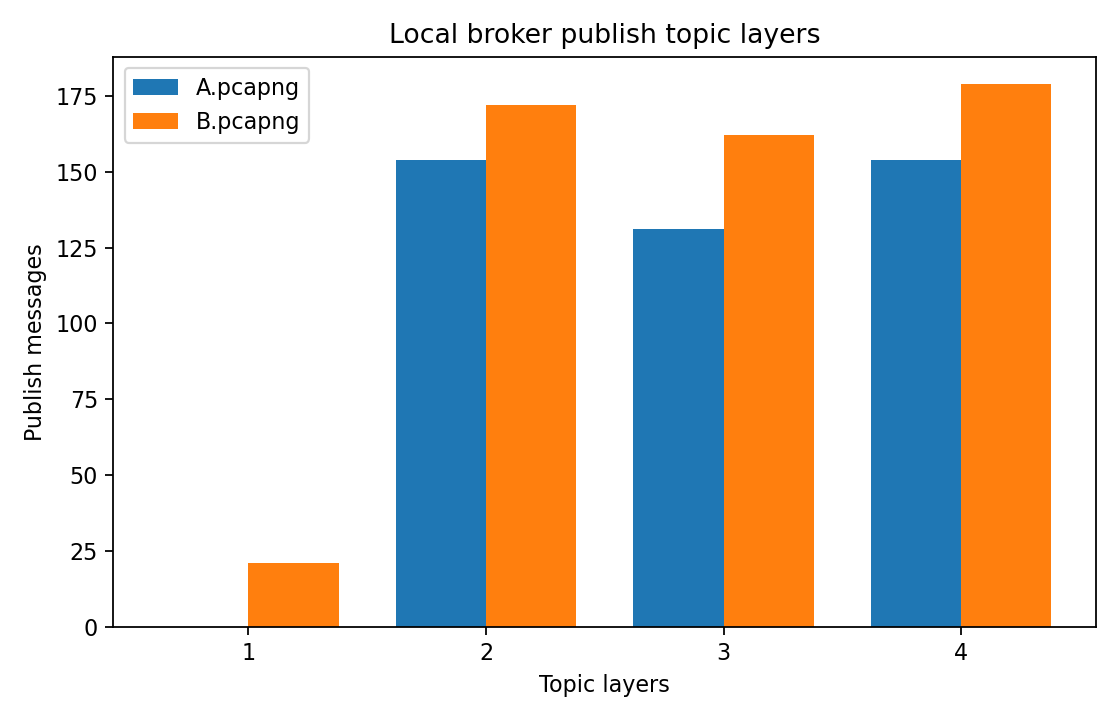
\includegraphics[width=0.85\linewidth]{cq8_histogram.png}
  \caption{Topic layer distribution for PUBLISH messages directed to the local broker.}
\end{figure}

\end{document}
